% Created 2023-03-04 sam. 20:01
% Intended LaTeX compiler: pdflatex
\documentclass[10pt,table,dvipsnames,compress]{beamer}
\usepackage[utf8]{inputenc}
\usepackage[T1]{fontenc}
\usepackage{graphicx}
\usepackage{longtable}
\usepackage{wrapfig}
\usepackage{rotating}
\usepackage[normalem]{ulem}
\usepackage{amsmath}
\usepackage{amssymb}
\usepackage{capt-of}
\usepackage{hyperref}
\usetheme{default}
\useinnertheme{rounded}
\useoutertheme[subsection=false]{miniframes}
\date{}
\title{\texttt{gecevar} R package -- GEt Climatic and Environmental VARiables}
\title[gecevar]{\texttt{gecevar} R package \\ GEt Climatic and Environmental VARiables}
\usepackage{lmodern}
\usepackage{pgf}
\usepackage{color}
\usepackage[english,french]{babel}
\setbeamertemplate{caption}[numbered]
\definecolor{vertmoyen}{RGB}{51,110,23} % vert moyen
\definecolor{blueFRB}{HTML}{31859c}
\usecolortheme[named=blueFRB]{structure}
\usepackage{tabularx} % varier la largeur du tableau
\usepackage{layout}
\setlength{\LTleft}{-5cm plus 1 fill}
\setlength{\LTright}{-5cm plus 1 fill}
\usepackage{booktabs}
\usepackage{arydshln} %% dashlines for tabular
\newcommand{\logit}{\text{logit}}
\newcommand{\bs}[1]{\boldsymbol{#1}}
\newcommand{\R}{\textnormal{\sffamily\bfseries R}}
\newcommand{\pkg}[1]{{\fontseries{b}\selectfont #1}}
\newcolumntype{C}[1]{>{\centering\arraybackslash}m{#1}}

\setbeamertemplate{footline}[frame number]
\setbeamertemplate{frametitle}{%
\usebeamerfont{frametitle}\insertframetitle%
\vphantom{g} % To avoid fluctuations per frame
\par
\centering 
\includegraphics[width=\textwidth]{figs/Barre_couleur}
}
\beamertemplatenavigationsymbolsempty

% Logo
\newif\ifplacelogo % create a new conditional
\logo{\ifplacelogo
\includegraphics[width=0.5\textwidth]{figs/partners_logos}\fi}

%Call table of contents at the beginning of each section
\AtBeginSection[]{
\placelogotrue
\begin{frame}
\frametitle{Plan}
\begin{columns}[c]
\begin{column}{0.5\textwidth}
\tableofcontents[sections=1,currentsection]
\vspace{0.5cm}
\tableofcontents[sections=2,currentsection]
\end{column}
\begin{column}{0.5\textwidth}
\tableofcontents[sections=3,currentsection]
\vspace{0.5cm}
\tableofcontents[sections=4,currentsection]
\end{column}
\end{columns}
\end{frame}
\placelogofalse
}

\AtBeginSubsection[]{}

\hypersetup{
colorlinks=true,
linkcolor=Black,
filecolor=Maroon,
citecolor=Blue,
urlcolor=Maroon}

% Disable monospaced font for URLs
\urlstyle{same}

\hypersetup{
 pdfauthor={Ghislain Vieilledent},
 pdftitle={\texttt{gecevar} R package -- GEt Climatic and Environmental VARiables},
 pdfkeywords={},
 pdfsubject={},
 pdfcreator={Emacs 28.2 (Org mode 9.6.1)}, 
 pdflang={English}}
\begin{document}


% Title page
{
  \setbeamertemplate{navigation symbols}{}
  \begin{frame}[plain, noframenumbering]
  
  \begin{center}
  \small{\textbf{AMAP -- METRADICA project -- March 2023}}
  \end{center}
  \vspace{-1cm}
  \titlepage % Presentation first page
  \vspace{-3.5cm}
  \begin{center}
    
\includegraphics[width=\textwidth]{figs/Barre_couleur}\\
    \vspace{0.5cm}
    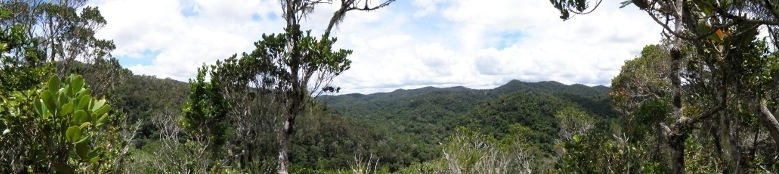
\includegraphics[width=10cm]{figs/Banniere}\\
    \vspace{0.3cm}
    \small{Jeanne CLEMENT$^{1}$\hspace{0.25cm}Ghislain VIEILLEDENT$^{1}$}\\
    \vspace{0.15cm}
    {\scriptsize
      \begin{tabular}{l}
        $[1]$ \textbf{Cirad} UMR AMAP
      \end{tabular}
    }\\
    \vspace{0.3cm}
    
\includegraphics[width=0.70\textwidth]{figs/partners_logos}
    
  \end{center}
  \end{frame}
}

% %%%%%%%%%%%%%%%%%%%%%%%%%%%%%%%%%%%%%%%%%%%%%%%%%%%%%%%%%%%%%%%%

\placelogotrue
\begin{frame}
  \frametitle{Plan}
  \begin{columns}[c]
    \begin{column}{0.5\textwidth}
      \tableofcontents[sections=1]
      \vspace{0.5cm}
      \tableofcontents[sections=2]
    \end{column}
    \begin{column}{0.5\textwidth}
        \tableofcontents[sections=3]
        \vspace{0.5cm}
        \tableofcontents[sections=4]
    \end{column}
  \end{columns}
\end{frame}
\placelogofalse

\section{Introduction}
\label{sec:orgda4b978}

\subsection{Context}
\label{sec:org2bb18b9}

\begin{frame}[label={sec:org4fc8ea7}]{Context}
\begin{itemize}
\item Ecology is the study of the relationships among living organisms and their physical environment.
\item Use of spatial environmental and climatic layers is inevitable in ecology.
\item (NB: Here, environmental variable = any environmental variable which is not climatic).
\item Study of the link between environment/climate and: species occurrence, species demography, individual traits, community characteristic (e.g. diversity, productivity, biomass, community weighted mean), etc.
\end{itemize}
\end{frame}

\begin{frame}[label={sec:orgb213867}]{Technically challenging steps}
\begin{itemize}
\item Several technical geoprocessing steps: crop to an extent, resample on a given grid (extent and resolution), combine data in one raster.
\item Some variables are missing and must be computed (number of dry months or average from climatic models).
\item Intensive computations if region is large and resolution is high (raster might not fit in memory).
\item Imply the use of technical geoprocessing software: R packages (terra, star, sf), gdal, GRASS GIS, Google Earth Engine.
\end{itemize}
\end{frame}

\begin{frame}[label={sec:org3c98f51}]{Time consuming and repetitive tasks}
\begin{block}{Time consuming}
\begin{itemize}
\item Many environmental variables (topography, soil, climate, land cover, disturbances, etc.).
\item Environment and climatic data are spread in different databases.
\item Long computations if region is large and resolution is high.
\item Downloading full rasters at global scale before cropping can take a lot of time.
\end{itemize}
\end{block}

\begin{block}{Repetitive}
\begin{itemize}
\item We usually repeat this work for every region we are working on.
\item For future climate data: repetition for each global climate model, scenario (SSP), and period (eg. 2055, 2085).
\end{itemize}
\end{block}
\end{frame}

\subsection{Objectives}
\label{sec:org21f5792}

\begin{frame}[label={sec:org955860c}]{Objectives}
\begin{itemize}
\item Provide an R package to ease the creation of a dataset with environmental and climatic variables for any particular region.
\item With easy-to-use and well documented functions.
\item Using efficient code and tools to fasten the creation of the dataset.
\end{itemize}
\end{frame}

\section{\texttt{gecevar} R package}
\label{sec:org12cea20}

\subsection{Functionalities}
\label{sec:orgc7790f8}

\begin{frame}[label={sec:orgc522286},fragile]{Functionalities}
 \begin{block}{Functions}
\begin{itemize}
\item \texttt{get\_env\_variables}: Raster file with 13 environmental variables.
\item \texttt{get\_chelsa\_current}: Raster file with 107 variables from Chelsa describing current climate (1980--2010).
\item \texttt{get\_chelsa\_future}: Raster file with 81 variables from Chelsa describing future climate (for each GCM, SSP, and period).
\end{itemize}
\end{block}

\begin{block}{Input}
By default, the user has to provide only one of the following:
\begin{itemize}
\item Country ISO code.
\item Shapefile with polygons delimiting the region of interest.
\item Extent (xmin, ymin, xmax, ymax) of the region of interest.
\end{itemize}
\end{block}
\end{frame}

\subsection{Variables}
\label{sec:org21bac8f}

\begin{frame}[label={sec:orgeef76fc}]{Environmental variables}
\begin{block}{Sources}
Various sources: SRTM, SoilGrids, Tropical Moist Forests, OpenStreetMap, WDPA. 
\end{block}

\begin{block}{Topography}
Elevation, Aspect, Slope, Roughness.
\end{block}

\begin{block}{Other environmental variables}
Solar irradiance, Soil, Forest cover, Distances to forest, sea, road, town, water, Protected areas.
\end{block}
\end{frame}

\begin{frame}[label={sec:org24570ac}]{Current climatic variables}
\begin{block}{Source}
Chelsa (\href{https://chelsa-climate.org)}{chelsa-climate.org})
\end{block}

\begin{block}{Bioclimatic variables}
\begin{itemize}
\item The monthly min, max and mean temperature and monthly precipitation (48 variables).
\item The 19 commonly used bioclimatic variables (11 from temperature and 8 from precipitation).
\end{itemize}
\end{block}

\begin{block}{Other climatic variables}
\begin{itemize}
\item Cloud area fraction, PET, Climatic water deficit (CWD), Number of dry months (NDM).
\item For PET and derived variables (CWD, NDM): Penman-Monteith or Thornthwaite equation.
\end{itemize}
\end{block}
\end{frame}

\begin{frame}[label={sec:org76bed84}]{Future climate}
\begin{block}{Source}
\begin{itemize}
\item Chelsa (\href{https://chelsa-climate.org)}{chelsa-climate.org})
\item GCMs: GFDL-ESM4, IPSL-CM6A-LR, MPI-ESM1-2-HR, MRI-ESM2-0, UKESM1-0-LL.
\item SSPs: Shared Socio-economic Pathways (126, 370, 585).
\item Periods: 2041--2070, 2071--2100.
\end{itemize}
\end{block}

\begin{block}{Future climate}
\begin{itemize}
\item Most of the climatic variables for each GCM, SSP, and period of time.
\item Exception: no Penman-Monteith PET and derived variables.
\item Averages from the 5 GCMs (ensemble model).
\end{itemize}
\end{block}
\end{frame}

\subsection{Specificities}
\label{sec:org76a3fd7}

\begin{frame}[label={sec:org5237fe0}]{Software used}
\end{frame}

\begin{frame}[label={sec:org8386f74}]{Cloud optimized GeoTIFFs (COGs)}
\end{frame}

\section{Case-studies}
\label{sec:org85a1fc3}

\subsection{Examples of computation time}
\label{sec:org38b475f}

\begin{frame}[label={sec:orge2f96ec}]{Examples of computation time}
\begin{table}[htbp]
\caption{\label{tab:org8290e49}Area size}
\centering
\small
\begin{tabular}{lll}
Area & raster size & nb. of cells\\[0pt]
\hline
Madagascar & 1673 x 875 & 1,463,875\\[0pt]
New Caledonia & 689 x 1921 & 1,323,569\\[0pt]
French Guiana & 444 x 445 & 197,580\\[0pt]
\end{tabular}
\end{table}

\begin{table}[htbp]
\caption{\label{tab:orgce68637}Computation time for 1km resolution}
\centering
\small
\begin{tabular}{lllll}
Area & env & clim current & merge files & clim future\\[0pt]
\hline
Madagascar & 13min & 25min & 6min & 1h15min\\[0pt]
New Caledonia & 5min & 9min & 8min & 47min\\[0pt]
French Guiana & 3min & 6min & 2min & 25min\\[0pt]
\end{tabular}
\end{table}
\end{frame}

\subsection{French Guiana}
\label{sec:org8a1229e}

\begin{frame}[label={sec:orgcdd2624}]{French Guiana}
\end{frame}

% %%%%%%%%%%%%%%%%%%%%%%%%%%%%%%%%%%%%%%%%%%%%%%%%%%%%%%%%%%

{
  % Use background image
  \usebackgroundtemplate{%
    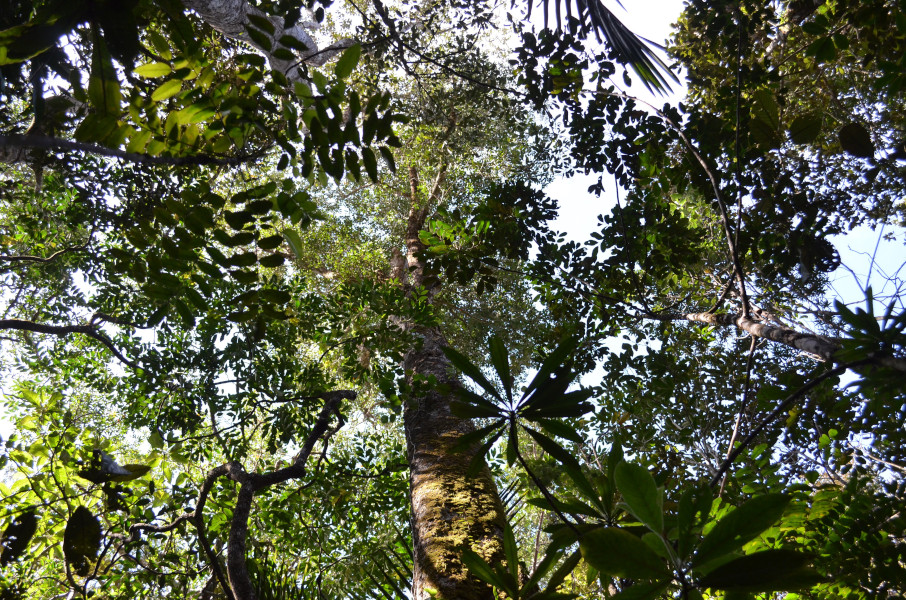
\includegraphics[keepaspectratio=true, height=\paperheight]{figs/Canopy-NC}
  }
  \setbeamertemplate{navigation symbols}{}
  % Remove shadow from block
  \setbeamertemplate{blocks}[rounded][shadow=false]
  \begin{frame}[plain]
  	\vspace*{\stretch{100}} 
    \begin{block}{}
      \begin{center}
        \ldots~Thank you for attention~\ldots \\
        \url{https://ecology.ghislainv.fr/presentations} \\
        
\includegraphics[width=0.55\textwidth]{figs/partners_logos}
      \end{center}
    \end{block}
  \end{frame}
}
\end{document}